\appendix
% RUN4-VERIFIED-APPENDIX: summaries generated from the archived MC20 CSVs.
\section{\edited{Reproducibility and seed stability}}\label{app:reproducibility}
{\color{red}{\color{black}
The empirical comparison uses a fixed curated real panel and four
synthetic panels, identified by the SHA-256 digests recorded in
\path{docs/panel_digests.txt}.}
The completed primary evaluation uses 100 matched inner draws,
200 ticker columns per draw, root seed 42, 200 outer corpus
replicates, and 20 independent inner-seed repeats.
Each metric--generator cell contains 200 valid outer scores and
20 valid seed-repeat scores, each calculated from 100 valid matched draws.
The point estimates in Table~\ref{tab:scores} use root seed 42;
they are not replaced by the mean across seeds.
Repeat zero reuses these estimates, and the other 19 seeds are derived
from an independent deterministic stream.
Tables~\ref{tab:mc-stability} and \ref{tab:mc-aggregate} report
the resulting mean, sample standard deviation, and observed range.
These summaries describe numerical variation conditional on the
observed corpora; they are not confidence intervals and do not include
generator retraining or regeneration.
In particular, AIL's M1 point estimate is $0.3436$, compared with
a seed mean of $0.3807$ and standard deviation $0.0131$.
This difference illustrates why the chosen point estimate and the
seed-stability distribution are reported separately.
The leading generator for each metric and the aggregate ordering
remain unchanged across all 20 seeds.
This is evidence about inner-resampling stability only, not
sensitivity to the metric specifications or to the choice of market period.
}

\begin{table}[htbp]
\centering
\color{red}
\caption{Per-metric numerical stability across $M=20$ inner-resampling seeds on fixed panels, with $R=100$ draws per seed. Ranges are observed minima and maxima, not confidence intervals.}
\label{tab:mc-stability}
\small
\begin{tabular}{@{}llcc@{}}
\toprule
Metric & Generator & Mean $\pm$ SD & Min--max \\
\midrule
M1 & AIL & $0.3807 \pm 0.0131$ & $[0.3436, 0.4021]$ \\
M1 & GBM & $0.0203 \pm 0.0010$ & $[0.0184, 0.0232]$ \\
M1 & MSV & $0.0864 \pm 0.0042$ & $[0.0790, 0.0983]$ \\
M1 & SBBTS & $0.0270 \pm 0.0014$ & $[0.0245, 0.0309]$ \\
\addlinespace
M2 & AIL & $0.2392 \pm 0.0141$ & $[0.2136, 0.2608]$ \\
M2 & GBM & $0.0209 \pm 0.0014$ & $[0.0184, 0.0234]$ \\
M2 & MSV & $0.3173 \pm 0.0169$ & $[0.2840, 0.3436]$ \\
M2 & SBBTS & $0.0228 \pm 0.0015$ & $[0.0201, 0.0255]$ \\
\addlinespace
M3 & AIL & $0.3632 \pm 0.0160$ & $[0.3298, 0.3932]$ \\
M3 & GBM & $0.1020 \pm 0.0052$ & $[0.0902, 0.1100]$ \\
M3 & MSV & $0.1308 \pm 0.0063$ & $[0.1155, 0.1424]$ \\
M3 & SBBTS & $0.2869 \pm 0.0118$ & $[0.2629, 0.3049]$ \\
\addlinespace
M4 & AIL & $0.4908 \pm 0.0166$ & $[0.4669, 0.5277]$ \\
M4 & GBM & $0.0389 \pm 0.0015$ & $[0.0362, 0.0428]$ \\
M4 & MSV & $0.0939 \pm 0.0035$ & $[0.0876, 0.1028]$ \\
M4 & SBBTS & $0.1256 \pm 0.0047$ & $[0.1154, 0.1362]$ \\
\bottomrule
\end{tabular}
\end{table}

\begin{table}[htbp]
\centering
\color{red}
\caption{Numerical stability of $G_{\mathrm{dev}}$ across the same 20 inner-resampling seeds.}
\label{tab:mc-aggregate}
\small
\begin{tabular}{@{}lcc@{}}
\toprule
Generator & Mean $\pm$ SD & Min--max \\
\midrule
AIL & $1.766 \pm 0.057$ & $[1.682, 1.911]$ \\
GBM & $26.523 \pm 0.781$ & $[25.014, 28.189]$ \\
MSV & $6.188 \pm 0.185$ & $[5.849, 6.561]$ \\
SBBTS & $12.794 \pm 0.390$ & $[12.025, 13.541]$ \\
\bottomrule
\end{tabular}
\end{table}

\clearpage
\section{\edited{Sensitivity grid}}\label{app:sensitivity}
{\color{red}
Figure~\ref{fig:sensitivity-scores} shows the mean score changes from the
same-seed primary specification over five seeds.
Figure~\ref{fig:sensitivity-aggregate} reports percentage changes in
aggregate deviation. M1 changes concern tail weighting of standardized
marginal returns; M4 changes concern volatility conditioning and tail shape.
The full numerical settings, seed-level results, coverage diagnostics,
and summary tables are recorded with the repository's sensitivity results.
Ranges across seeds are numerical diagnostics, not corpus confidence intervals.
}
\begin{table}[htbp]
\centering
\color{red}
\caption{Ranges of paired changes from the same-seed primary across the tested alternatives and five seeds. M1 and M4 entries are score differences; aggregate entries are percentage changes in $G_{\mathrm{dev}}$. These minima and maxima are not confidence intervals.}
\label{tab:sensitivity-ranges}
\small
\begin{tabular}{@{}lccc@{}}
\toprule
Generator & M1 change & M4 change & $G_{\mathrm{dev}}$ change (\%) \\
\midrule
AIL & $[-0.0452, 0.0144]$ & $[-0.0378, 0.0181]$ & $[-1.80, 5.08]$ \\
GBM & $[-0.0008, 0.0009]$ & $[-0.0086, 0.0072]$ & $[-4.45, 6.74]$ \\
MSV & $[-0.0140, 0.0058]$ & $[-0.0240, 0.0149]$ & $[-4.08, 8.56]$ \\
SBBTS & $[-0.0006, 0.0017]$ & $[-0.0121, 0.0168]$ & $[-3.75, 3.00]$ \\
\bottomrule
\end{tabular}
\end{table}

\begin{figure}[htbp]
\centering
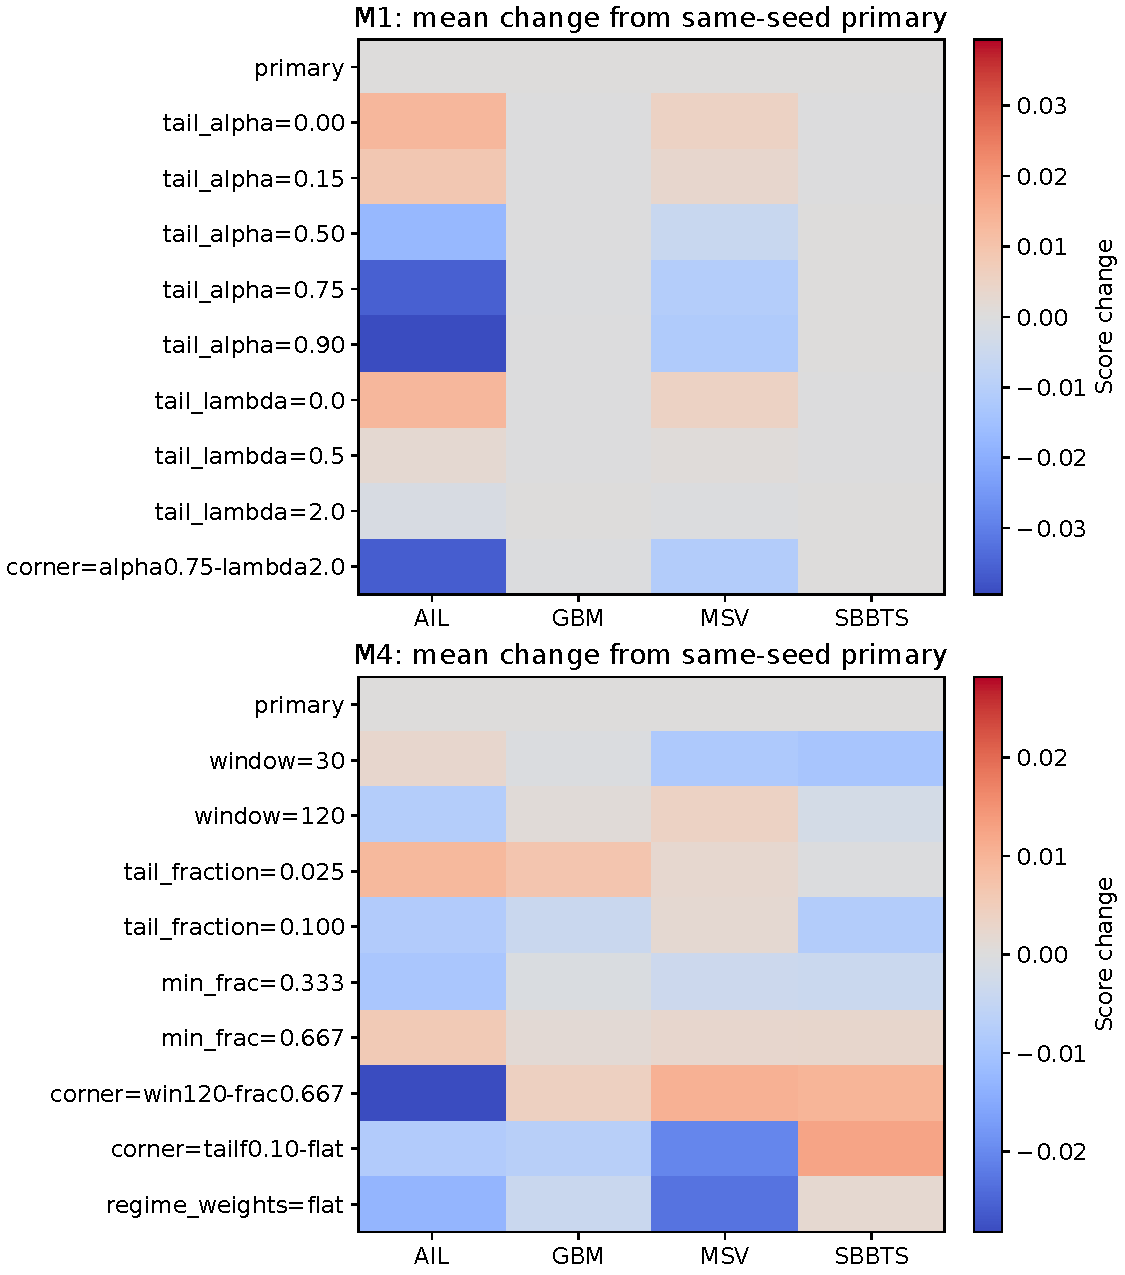
\includegraphics[width=\textwidth]{figures/sensitivity_scores.pdf}
\caption{\edited{Mean change in M1 and M4 scores from the same-seed primary,
over five seeds. Each panel shows the primary and the nine alternatives
affecting that metric; fixed M2 and M3 settings are omitted.}}
\label{fig:sensitivity-scores}
\end{figure}
\begin{figure}[htbp]
\centering
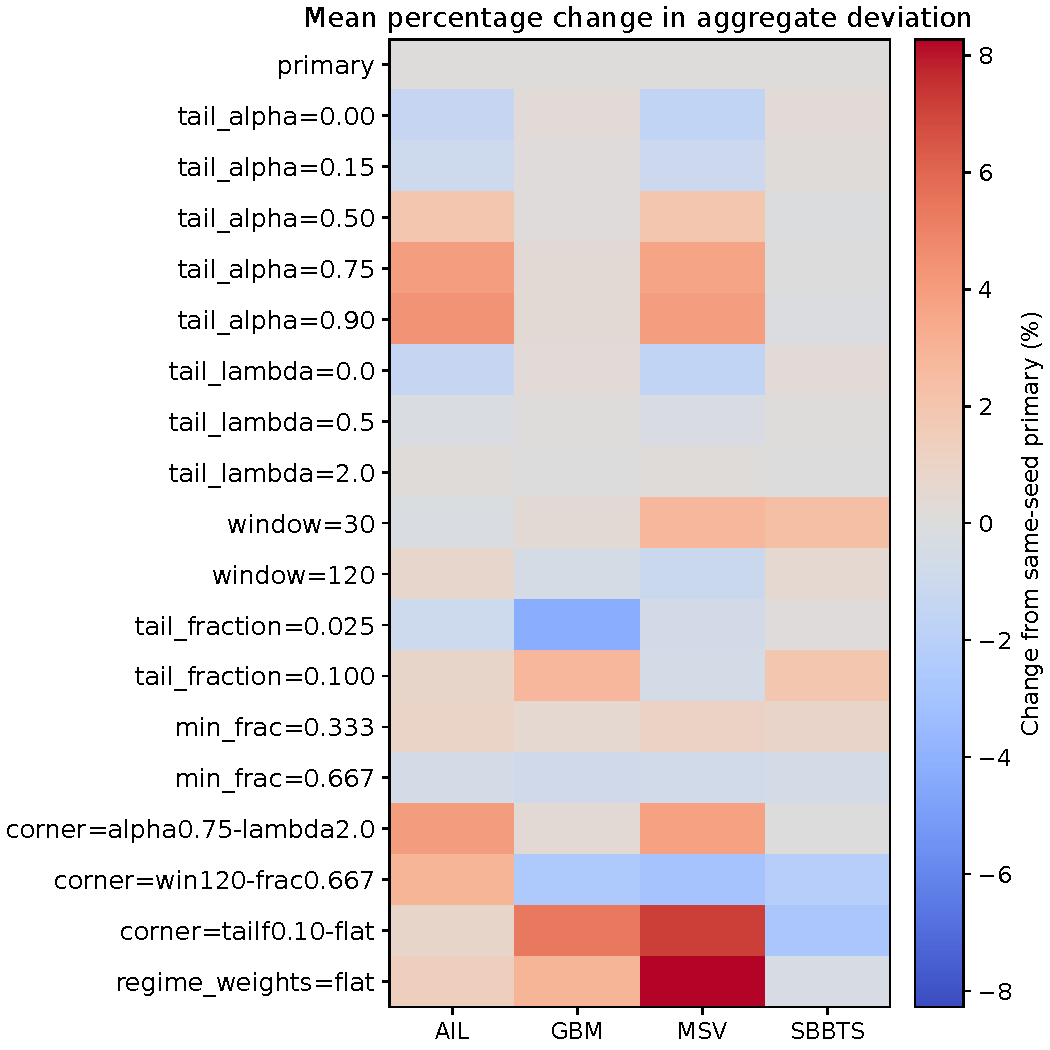
\includegraphics[width=\textwidth]{figures/sensitivity_aggregate.pdf}
\caption{\edited{Mean percentage change in aggregate deviation from the
same-seed primary. Lower aggregate deviation indicates closer gap parity.}}
\label{fig:sensitivity-aggregate}
\end{figure}

